\part{Seminar 2 - Simple Analytical Expressions for the Force and Torque of Axial Magnetic Couplings}

\makebox[.25\textwidth]{Louis Colin}\makebox[.25\textwidth]{Charles Dubuc}\makebox[.25\textwidth]{Clément Martin}\makebox[.25\textwidth]{Guillaume Percy}

\section{Theoritical reminders}


Let's remind some magnetic elements useful in our presentation : 

\begin{itemize}
    \item $\vec{M}$ : magnets magnetization
    \item $\vec{H}$ : magnetic excitation
      \item $\vec{B}$ : magnetic induction, with $B = \mu_0(\vec{H}+\vec{M})$
    
\end{itemize}


In order to determine the 2 following boundary conditions : 


\begin{equation*}
\left\{
    \begin{array}{l}
    \hat{n}\cdot(\vec{B}_1 - \vec{B}_2) = 0 
       \\
        \hat{n}\times (\vec{H}_1 - \vec{H}_2) = 0 
    \end{array}
\right.    
\end{equation*}

We will need the following Maxwell equations : 

\begin{equation*}
\left\{
    \begin{array}{ll}
     \nabla \times \vec{H} = \dfrac{\partial \vec{D}}{\partial t} + \vec{J} & \text{Ampere Law}
       \\
         \nabla \cdot \vec{B} = 0 & \text{Gauss Law for magnetism}
    \end{array}
\right.
\end{equation*}

Since there is no electric field in our problem and no current, the Ampere Law becomes : 

\begin{equation*}
\left\{
    \begin{array}{ll}
     \nabla \times \vec{H} =0 & \text{Ampere Law}
       \\
         \nabla \cdot \vec{B} = 0 & \text{Gauss Law for magnetism}
    \end{array}
\right.    
\end{equation*}

\subsubsection*{First boundary condition}

Let's use the Gauss Law for magnetism, then integrate it on a closed volume. By using the divergence theorem, this integral becomes a closed surface integral : 

\begin{equation*}
    \nabla \cdot \vec{B} = 0 ~~~~~~~~~ \iiint_V \nabla\cdot \vec{B} dV = 0 ~~~~~~~\iint_S \vec{B}\cdot \hat{n}dS = 0 ~~~~
\end{equation*}

With 

\begin{equation*}
     \left\{
    \begin{array}{ll}
    \vec{B} = \vec{B}_1 & \text{Zone 1} \\
    \vec{B} = \vec{B}_2 & \text{Zone 2} \\
    \end{array}
\right.
\end{equation*}


\begin{figure}[H]
    \centering
    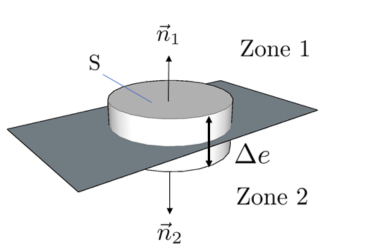
\includegraphics[scale=0.5]{Bound1.png}
    \caption{Geometry of the first boundary condition}
\end{figure}

We integrate it on the closed surface which is an infinitesimal cylinder between two zones : 
\begin{equation*}
    \vec{B}_1\cdot\hat{n}_1\cdot S+ \vec{B}_2\cdot\hat{n}_2\cdot S + \text{Lateral Contribution} = 0
    \end{equation*}
  Since we consider that the cylinder is infinitesimal, $ \Delta e \rightarrow 0$, the lateral contribution tends also to 0 :
    \begin{equation*}
    (\vec{B}_1\cdot\hat{n}_1+ \vec{B}_2\cdot\hat{n}_2)\cdot S = 0  \end{equation*}
    And as the two normal vectors are equal but opposite : 
    \begin{equation*}
    \vec{n}_1 = -\vec{n}_2 = \vec{n}
\end{equation*}
    We find the following relations which physically means that we have the continuity of the tangential component of magnetic field B. 
\begin{equation*}
    \boxed{(\vec{B}_1 - \vec{B}_2)\cdot \hat{n} = 0 }
\end{equation*}

   \subsubsection*{Second boundary condition}
   By using the infinitesimal Ampere Law, integrating it on a surface and using the Stokes theorem to have a closed single integral on a closed contour : 
   
   \begin{equation*}
       \nabla \times \vec{H} =0  ~~~~ \iint_S  \nabla \times \vec{H} dS  ~~~  \oint_C \vec{H}\cdot \vec{dl} = 0
   \end{equation*}
   
   
 \begin{figure}[H]
     \centering
     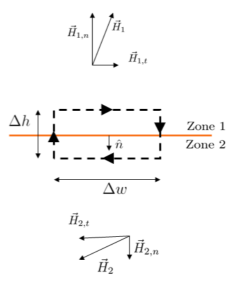
\includegraphics[scale=0.6]{Bound2.png}
     \caption{Geometry of the second boundary condition}
 \end{figure}
 
 We integrate the magnetic field $\vec{H}$ on a closed rectangle between two zones, and have the following equation :
 
 \begin{equation*}
       \oint \vec{H} \cdot \vec{dl} =  H_{1,t}\Delta w  + H_{1,n}\frac{\Delta h}{2}  + H_{2,n}\frac{\Delta h}{2} - H_{2,t}\Delta w - H_{2,n}\frac{\Delta h}{2}  - H_{1,n}\frac{\Delta h}{2} = 0
   \end{equation*}
   Some terms cancel each other, and it only remains : 
   \begin{equation*}
        \oint_C \vec{H}\cdot \vec{dl} = 0 =  H_{1,t}\Delta w- H_{2,t}\Delta w = 0
   \end{equation*}
Since the tangential component of this problem is equal to the cross product between the field and the normal of the interface, we obtain the second boundary condition : 
   \begin{equation*}
       \vec{H}_{1,t} - \vec{H}_{2,t} = 0 ~~~~~= \boxed{(\vec{H}_1 - \vec{H}_2) \times \hat{n}}
          \end{equation*}





\section{Problem description and assumptions}

\begin{figure}[H]
    \centering
    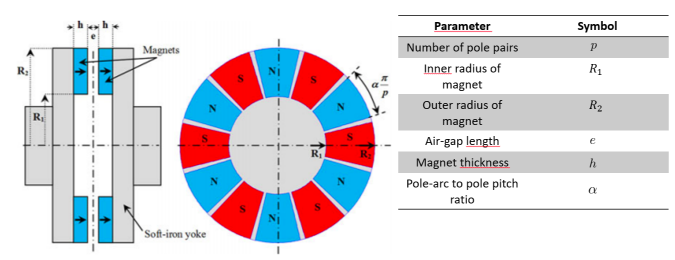
\includegraphics[scale=0.4]{desrciption.png}
\end{figure}

Comment about the previous figure : $\alpha$ can be seen as the percentage of magnet perimeter (at r = $R_2$) compared to whole circle ($2\pi R_2$). 

\bigskip

In order to make an easier analyse of the problem, the idea is to switch from a 3D to a 2D problem. This can be done by doing several assumptions : 

\begin{itemize}
    \item Radial component of the magnetic field neglected, because we will work a one particular radius $R_e = \frac{R_1 + R_2}{2}$
    \item Axial and tangential components independent of $r$ coordinate
    \item In the iron yokes : $\mu = \infty$
    \item The magnets are axially magnetized with $\mu_r = 1$
\end{itemize}

With help of the demonstration for proving the shape of the vector potential $\Bar{A}(\theta,z)$ in appendix \ref{apdxC}, all these assumptions give for the magnetic field and the vector potential respectively :

\begin{figure}[H]
    \centering
  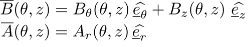
\includegraphics[scale=0.4]{B+A.png}
\end{figure}

Now, to pass from 3D to 2D problem, the unrolling of the two cylinders is made like this :

\begin{figure}[H]
    \centering
  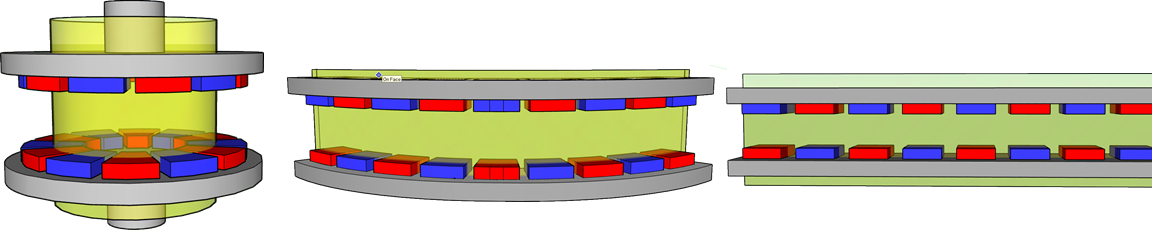
\includegraphics[scale=0.5]{Deroule.png}
\end{figure}

Then , the two faces of the cylinders are seen as two infinite plates.

\bigskip

Finally, the last thing to do is to create the new coordinate frame that will be used for calculations. As a reminder, a cutting surface is creating at $R_e = \frac{R_1 + R_2}{2}$, as illustrated on the following figure : 


\begin{figure}[H]
    \centering
    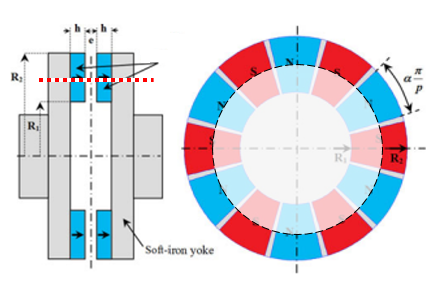
\includegraphics[scale=0.8]{cut_surf.png}
\end{figure}

As a result, the region analysed will be of the following shape : 

\begin{figure}[H]
    \centering
    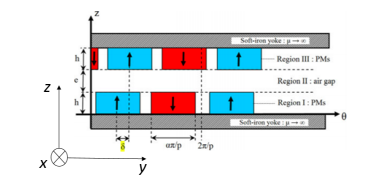
\includegraphics[scale=0.7]{shape.png}
\end{figure}

There are two last comments to make : 
\begin{itemize}
    \item The frame (x,y,z) comes from the following transformation : 

\begin{figure}[H]
    \centering
    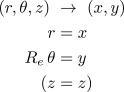
\includegraphics[scale=0.45]{frame.png}
\end{figure}

\item The variable $\delta$ is important, and refers to the sliding angle difference between the two cylinders. Further, it will depend on the load applied on two shafts.
\end{itemize}


\section{2-D analytical model}

\subsection*{Derivation of the problem governing equations}

Let's remind the fundamental equations we will need :
\begin{align*}
    \overline{\nabla} \times \overline{H} &= \overline{0} &
    \overline{B} &= \mu_0\, ( \overline{H} + \overline{M} ) &
    \overline{B} &= \overline{\nabla} \times \overline{A}
\end{align*}

Using these relations, we can find :
\begin{align*}
\overline{\nabla} \times \left( \dfrac{\overline{B}}{\mu_0} - \overline{M} \right) &= \overline{0} \\
\overline{\nabla} \times \overline{B} &= \mu_0\, \overline{\nabla} \times \overline{M} \\
\overline{\nabla} \times \left( \overline{\nabla} \times \overline{A} \right) &= \mu_0\, \overline{\nabla} \times \overline{M} \\
- \overline{\nabla}^2 \overline{A} + \overline{\nabla} \left( \overline{\nabla} \cdot \overline{A} \right) &= \mu_0\, \overline{\nabla} \times \overline{M} 
\end{align*}

The potential vector being defined up to a gradient, we can arbitrarily choose the value of $\overline{A}$. We decide here to choose it such that $\overline{\nabla} \cdot \overline{A} = 0$. As $\overline{M}$ is null in the air gap region (\rm II), we get :

\begin{equation}
\label{eq:regions}
\left\{
 \begin{array}{lr}
\overline{\nabla}^2 \overline{A} = - \mu_0\, \overline{\nabla} \times \overline{M} 
& \text{regions \rm I and \rm III} \\
\overline{\nabla}^2 \overline{A} = 0 
& \text{region \rm II}
 \end{array}
\right. 
\end{equation}

We can further develop these relations knowing that the $\overline{A}$ and $\overline{M}$ vectors are of the following form :
\begin{align*}
    \overline{A} &= A_r (\theta, z) \widehat{\underline{e}_r} &
    \overline{M} &= \pm \dfrac{B_r(\theta)}{\mu_0}\widehat{\underline{e}_z}
\end{align*}
We remind that our problem is developed in the Cartesian frame and not the cylindrical one. This means that we have a simple change of variable to do if we want to use the classical notations $x,y,z$ instead of $r,\theta,z$ :
\begin{align}
\label{eq:change_vars}
    r &= x &
    R_e\, \theta &= y &
    z &= z
\end{align}
We then have new writing for  :
\begin{align*}
     \overline{A} &= A_x (y, z) \widehat{\underline{e}_x} &
    \overline{M} &= \pm \dfrac{B_r(y)}{\mu_0}\widehat{\underline{e}_z}
\end{align*}

Developing the expression of $\overline{\nabla}^2 \overline{A}$ and $\overline{\nabla} \times \overline{M}$ in the Cartesian frame :
\begin{align*}
\overline{\nabla}^2 \overline{A} &= \left( \dfrac{\partial ^2 A_x}{\partial x^2}\underbrace{ + \dfrac{\partial ^2 A_x}{\partial y^2} + \dfrac{\partial ^2A_x}{\partial z^2}}\right) \widehat{\underline{e}_x}+ \left( \dfrac{\partial ^2 A_y}{\partial x^2} + \dfrac{\partial ^2A_y}{\partial y^2} + \dfrac{\partial ^2 A_y}{\partial z^2}\right)\widehat{\underline{e}_y}+ \left( \dfrac{\partial ^2A_z}{\partial x^2} + \dfrac{\partial ^2 A_z}{\partial y^2} +\dfrac{\partial ^2 A_z}{\partial z^2}\right)\widehat{\underline{e}_z}\\
&= \qquad \left( \dfrac{\partial ^2 A_r}{\partial \theta^2}\,\dfrac{1}{R_e^2} + \dfrac{\partial ^2 A_r}{\partial z^2}\right)\widehat{\underline{e}_r} \\
\overline{\nabla} \times \overline{M} &= \left( \underbrace{ \dfrac{\partial M_z}{\partial y} }- \dfrac{\partial M_y}{\partial z} \right) \widehat{\underline{e}_x} + \left( \dfrac{\partial M_x}{\partial z} - \dfrac{\partial M_z}{\partial x} \right) \widehat{\underline{e}_y} +\left( \dfrac{\partial M_y}{\partial x} - \dfrac{\partial M_x}{\partial y} \right) \widehat{\underline{e}_z} \\
&= \dfrac{\partial M_z}{\partial \theta}\, \dfrac{1}{R_e} \widehat{\underline{e}_r}
\end{align*}
Wrapping up the last two equations into relation (\ref{eq:regions}), we get the problem Poisson and Laplace equations that need to be solved to get compute the $\overline{A}$ and thus the $\overline{B}$ field:
\begin{align}
\dfrac{1}{R_e^2}\, \dfrac{\partial^2 A}{\partial \theta ^2} +\dfrac{\partial^2 A}{\partial z^2} &= -\dfrac{\mu_0}{R_e}\, \dfrac{\partial M_z}{\partial \theta} \hspace{.2cm} &\text{for} \left\{ \begin{array}{l}  h+e \leq z \leq 2h+e \hspace{.2cm} \text{for region \rm III} \hspace{.2cm} \text{or}\hspace{.2cm} 0 \leq z \leq h \hspace{.2cm} \text{for region \rm I}\\ 
 0 \leq \theta \leq 2\pi/p 
\end{array}
\right. \\
\dfrac{1}{R_e^2}\, \dfrac{\partial^2 A}{\partial \theta ^2} +\dfrac{\partial^2 A}{\partial z^2} &= 0   &\text{for} \left\{ \begin{array}{l}  h \leq z \leq h+e \hspace{.2cm} \text{for region \rm II} \hspace{.2cm}\\  0 \leq \theta \leq 2\pi/p 
\end{array}
\right. 
\end{align}



\subsection*{Derivation of the problem boundary conditions}

Here are as a reminder the boundary conditions our problem should respect between interfaces of different regions
\begin{align*}
\overline{n}_{12} \times \left( \overline{H}_2 - \overline{H}_1 \right) &= \overline{0} &
\overline{n}_{12} \cdot \left( \overline{B}_2 - \overline{B}_1 \right) &= 0 
\end{align*}
As we will further solve the Poisson equation in region \rm III, we will here develop the boundary conditions for \rm III.
\begin{figure}[H]
    \centering
    \begin{minipage}[b]{0.58\linewidth}
        \begin{align*} 
        n_{12}\ \widehat{\underline{e}}_z \times \left( H_{2z}\ \widehat{\underline{e}}_z + H_{2\theta}\ \widehat{\underline{e}}_{\theta} \right) &=  n_{12}\ \widehat{\underline{e}}_z \times \left( H_{1z}\ \widehat{\underline{e}}_z + H_{1\theta}\ \widehat{\underline{e}}_{\theta} \right) \\ -n_{12}\, H_{2\theta}\, \widehat{\underline{e}}_r &= -n_{12}\, H_{1\theta}\, \widehat{\underline{e}}_r \\ 
        H_{2\theta} &= H_{1\theta} \\
        H_{\theta}^{\rm III} &= H_{\theta}^{\rm II }
\end{align*}
Same reasoning can be done over the second boundary condition so that we finally get :
\begin{align}
\label{eq:BC1}
\overline{H}_{\theta}^{\rm III} &= \overline{H}_{\theta}^{\rm II} &
\overline{B}_z^{\rm III} &= \overline{B}_z^{\rm II} 
\end{align}
    \end{minipage}%%%
    \begin{minipage}[b]{0.4\linewidth}
    \flushright
    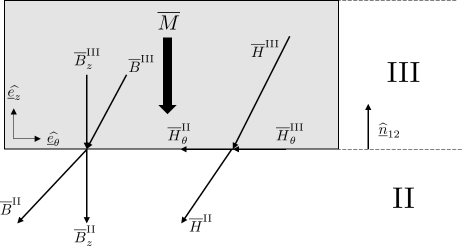
\includegraphics[width=.9\textwidth]{BC.png}
    \end{minipage}
    %\hspace*{-4cm}
\end{figure}

In order to go further in the developing of the boundary conditions, we shall need new relations derived from the expression of $\overline{B}$. We have :
\begin{align*}
    \overline{B} &= \overline{\nabla} \times \overline{A} &
    \overline{A} &= A_r (\theta, z) \widehat{\underline{e}_r}
\end{align*}
In the Cartesian frame, the first relation translates as :
$$
B_x\ \widehat{\underline{e}_x} + B_y\ \widehat{\underline{e}_y} + B_z\ \widehat{\underline{e}_z} = \left( \dfrac{\partial A_z}{\partial y} - \dfrac{\partial A_y}{\partial z} \right) \widehat{\underline{e}_x} +  \left( \dfrac{\partial A_x}{\partial z} - \dfrac{\partial A_z}{\partial x} \right) \widehat{\underline{e}_y} + \left( \dfrac{\partial A_y}{\partial x} - \dfrac{\partial A_x}{\partial y} \right) \widehat{\underline{e}_z}$$
using the change of variable (\ref{eq:change_vars}) we get
$$B_r\ \widehat{\underline{e}_r} + B_{\theta}\ \widehat{\underline{e}_{\theta}} + B_z\ \widehat{\underline{e}_z} = \left( \dfrac{\partial A_z}{\partial \theta}\, \dfrac{1}{R_e} - \dfrac{\partial A_{\theta}}{\partial z} \right) \widehat{\underline{e}_r} +  \left( \dfrac{\partial A_r}{\partial z} - \dfrac{\partial A_z}{\partial r} \right) \widehat{\underline{e}_{\theta}} + \left( \dfrac{\partial A_{\theta}}{\partial r} - \dfrac{\partial A_r}{\partial \theta}\, \dfrac{1}{R_e} \right) \widehat{\underline{e}_z}$$
This relation simplifies to finally give
 $$\dfrac{\partial A_r}{\partial z} = B_{\theta} \hspace{4cm}  - \dfrac{\partial A_r}{\partial \theta}\ \dfrac{1}{R_e} = B_z$$
The last two relations will be extremely useful as we will use them to get $\overline{B}$ once we will have find $\overline{A}$.\\
Using these relations as well as (\ref{eq:BC1}), we find :
\begin{align}
\label{eq:linkAB}
\dfrac{\partial A_{\rm II}}{\partial \theta} &= 
\dfrac{\partial A_{\rm III}}{\partial \theta} &
\dfrac{\partial A_{\rm II}}{\partial z} &= 
\dfrac{\partial A_{\rm III}}{\partial z} \\
A_{\rm II} &= A_{\rm III} + C_1(z) &
A_{\rm II} &= A_{\rm III} + C_2(\theta)
\end{align}
$\cdot$ \underline{at interface $z = h+e$}
\begin{equation}
\label{eq:BC2_1}
A_{\rm II}(\theta,\ h+e) = A_{\rm III}(\theta,\ h+e)    
\end{equation}
$\cdot$ \underline{at interface $z = 2h+e$}
\begin{align*}
    B_{\theta} = \underbrace{\mu}_1\ H_{\theta} = 0 &= \dfrac{\partial A_r}{\partial z} \\
    \dfrac{\partial A_{\rm III}}{\partial z}\Bigr\rvert_{z = 2h+e} &= 0 \numberthis \label{eq:BC2_2}
\end{align*}

Equations (\ref{eq:BC2_1}) and (\ref{eq:BC2_2}) finally constitute the boundary conditions we need to meet while solving the Poisson equation in region \rm III. 

\subsection*{Problem solving in region III}

To sum up, the problem to solve in region \rm III is the following :
\begin{equation}
\label{eq:PoissonIII}
 \dfrac{1}{R_e^2}\, \dfrac{\partial^2 A_{\rm III}}{\partial \theta ^2}
+ \dfrac{\partial^2 A_{\rm III}}{\partial z^2}
= -\dfrac{\mu_0}{R_e}\, \dfrac{\partial M_z}{\partial \theta}
\hspace{.5cm} \text{for}
\left\{
\begin{array}{lll}
& h+e \leq z \leq 2h+e \\
& 0 \leq \theta \leq 2\pi/p
 \end{array}
\right.
\end{equation}
As the problem is periodic, the magnetization vector can be developed using Fourier series :

\begin{figure}[H]
    \centering
    \begin{minipage}[b]{0.5\linewidth}
     \flushleft
    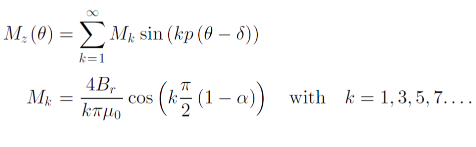
\includegraphics[width=.9\textwidth]{Mz.png}
    \vspace{1.5cm}
    \end{minipage}%%%
    \begin{minipage}[b]{0.45\linewidth}
    \flushright
    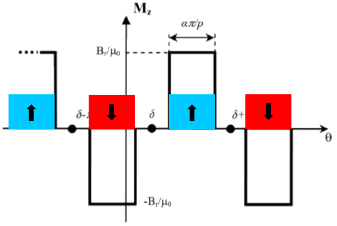
\includegraphics[width=.9\textwidth]{Mz_graph.png}
    \end{minipage}
    %\hspace*{-4cm}
\end{figure}

This problem is solved using variable separations presented in appendix \ref{apdxA}. Fourier series expansion are used to find coefficient values. A reminder of this technique is also given in the same appendix. The final result in region \rm III is found as :
\begin{align*}
A_{\rm III} (\theta, z) 
&= \sum\limits_{k=1}^{\infty}\Bigr( \cosh \bigr((kp/R_e)\, (z-2h-e)\bigr) \Bigr)\,
d_k + K_k\, \cos(kp\delta) \Bigr)\, \cos(kp\theta) \\
&+ \sum\limits_{k=1}^{\infty}\Bigr( \cosh \bigr((kp/R_e)\, (z-2h-e)\bigr) \Bigr)\,
e_k + K_k\, \sin(kp\delta) \Bigr)\, \sin(kp\theta)
\end{align*}
Relations (\ref{eq:linkAB}) are then used to finally determine the analytical expression of the magnetic field.




\section{Axial Force and Torque expressions}

Now we have an analytical expression for the vector potential $\mathbf{A}$, let's use it in order to compute the axial force and the torque expression. 

\subsection*{Maxwell Stress tensor}

The tool we will use to compute forces and torque is Maxwell Stress tensor. It is \textit{ is a symmetric second-order tensor used in classical electromagnetism to represent the interaction between electromagnetic forces and mechanical momentum}. Here is its expression : 

\begin{align*}
T_{ij} = \dfrac{B_iB_j}{\mu_0} - \delta_{ij}\dfrac{|\mathbf{B}|^2}{2\mu_0} + \epsilon_0 E_i E_j - \dfrac{1}{2}\epsilon_0|\mathbf{E}|^2 \delta_{ij}
\end{align*}

Since we only have magnetic fields in our problem, and no electric field, the expression is reduced to :

\begin{equation*}
T_{ij} = \dfrac{B_iB_j}{\mu_0} - \delta_{ij}\dfrac{|\mathbf{B}|^2}{2\mu_0} 
\end{equation*}

Here is what it gives in term of matrix : 

\begin{equation*}
\mathbf{T} =  \dfrac{1}{\mu_0}
\begin{bmatrix}
\dfrac{B_r^2 - B_{\theta}^2 - B_z^2}{2} & B_rB_{\theta} & B_rB_z \\
B_{\theta}B_r & \dfrac{B_{\theta}^2 - B_r^2 - B_z^2}{2} & B_{\theta}B_z \\
B_zB_r & B_zB_{\theta} & \dfrac{B_z^2 - B_r^2 - B_{\theta}^2}{2}\\
\end{bmatrix}
\end{equation*}

But since we established previously that magnetic field has only two components, with 2 variables : 

\begin{equation*}
    \mathbf{B} = B_{\theta}(\theta,z)\mathbf{e_{\theta}}+B_z(\theta,z)\mathbf{e_z} 
\end{equation*}

The tensor can be simplified as follows :

\begin{equation*}
\mathbf{T} = \dfrac{1}{\mu_0}
\begin{bmatrix}
 - \dfrac{B_{\theta}^2 + B_z^2}{2} &0 & 0  \\
0 & \dfrac{B_{\theta}^2 - B_z^2}{2} & B_{\theta}B_z \\
0 & B_zB_{\theta} & \dfrac{B_z^2 - B_{\theta}^2}{2}\\
\end{bmatrix}
\end{equation*}


\subsection*{Surface of integration}
\begin{figure}[H]
   \begin{minipage}[b]{.66\linewidth}

As we saw in previous courses, we can find the forces in the air gap by integrating the Maxwell on a closed surface, such as the following equation :  
\begin{equation*}
\vec{F} = \oint_S \mathbf{T}\cdot \vec{n} dS
\end{equation*}
   The chosen closed surface can be considered as a cylinder of infinite radius.
\end{minipage} \hfill
   \begin{minipage}[b]{.26\linewidth}
      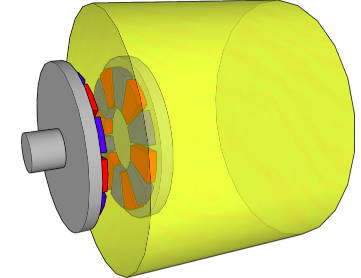
\includegraphics[scale=0.3]{CSurface1.png}
          \label{CS1}
   \end{minipage}
\end{figure}

\begin{figure}[H]
\begin{minipage}[b]{.7\linewidth}
Since we considered that magnetic field only no radial component, the integration on the lateral surface has no contribution. The back surface of the cylinder also has no contribution since there is no more magnetic field behind the two "plates". Finally, the only area where magnetic field has non-negligible components is between $R_1$ and $R_2$. The remaining area simplifies into a "pineapple slice". The normal to this surface is along $\hat{e}_z$, and can be represented as :
\begin{equation*}
\vec{n} = \mathbf{e_z} =  \begin{bmatrix}
 0  \\ 0 \\ 1 
\end{bmatrix}   
\end{equation*}
\textbf{It's important to notice that we integrate in the air gap, in zone II.}
\end{minipage}
\hfill
\begin{minipage}[b]{.2\linewidth}
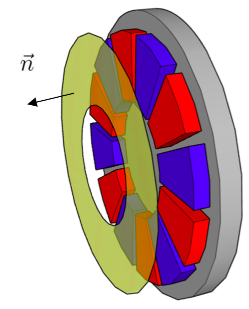
\includegraphics[scale=0.3]{CSurface2.png}
\end{minipage}
\end{figure}

\subsection*{Tangential force and torque expression}

Starting from this, we can multiply the Maxwell Stress Tensor by the normal to get the infinitesimal force in the air gap, which has 3 components in $\hat{e}_r,\hat{e}_{\theta}$ and $\hat{e}_z$, and we can see that there is no radial component of the force.  

\begin{equation*}
    \mathbf{T} \cdot \vec{n} = \dfrac{1}{\mu_0}\begin{bmatrix}
 - \dfrac{B_{\theta}^2 + B_z^2}{2} &0 & 0  \\
0 & \dfrac{B_{\theta}^2 - B_z^2}{2} & B_{\theta}B_z \\
0 & B_zB_{\theta} & \dfrac{B_z^2 - B_{\theta}^2}{2}\\
\end{bmatrix}
 \begin{bmatrix}
 0  \\ \\ 0 \\ \\ 1 
\end{bmatrix}    = \dfrac{1}{\mu_0}
\begin{bmatrix}
 0 \\ \\ B_z B_{\theta} \\ \\ \dfrac{B_z^2-B^2_{\theta}}{2}
\end{bmatrix}
\end{equation*}
\vspace{0.5cm}
In order to compute the torque, we first have to compute the component of the force which creates the torque. It is the tangential one, $F_{\theta}$. We have to integrate it on the hollowed disk discussed before, so from $r=R_1$ to $r=R_2$, and from $\theta = 0$ to $\theta = 2\pi$ because we make the whole revolution of the disk. 
\vspace{0.5cm}
\begin{equation*}
F_{\theta} = \dfrac{1}{\mu_0}\oint_S B_{IIz}(\theta,z)B_{II\theta}(\theta,z) dS = \dfrac{1}{\mu_0}\int_0^{2\pi}\int_{R_1}^{R_2}B_{IIz}(\theta,z)B_{II\theta}(\theta,z)rdrd\theta
\end{equation*}
\vspace{0.5cm}
Since the lever arm is perpendicular to $F_{\theta}$, the cross product $\vec{r} \times \vec{F}$ becomes $rF_{\theta}$ : 

     \begin{align*}
 T_e = rF_{\theta}  &=  \dfrac{1}{\mu_0}\int_0^{2\pi}\int_{R_1}^{R_2}B_{IIz}(\theta,z)B_{II\theta}(\theta,z)r^2drd\theta   \\
&= \dfrac{1}{\mu_0}\int_0^{2\pi}B_z(\theta,z)B_{\theta}(\theta,z)d\theta\int_{R_1}^{R_2}r^2dr   \\
&= \dfrac{R_2^3-R_1^3}{3\mu_0}\int_0^{2\pi}B_z(\theta,z)B_{\theta}(\theta,z)d\theta
\end{align*}
     
Now we have to integrate the product of the 2 components of the magnetic field. In order to compute that, we will use the results previously derived : 
\begin{align*}
 \dfrac{\partial A_r}{\partial z} &= B_{\theta} \hspace{4cm}  - \dfrac{\partial A_r}{\partial \theta}\ \dfrac{1}{R_e} = B_z
\end{align*}

With the following expression for A in region II : 

\begin{align*}
    A_{II}(\theta,z) &= \sum_{k=1}^{\infty} \left(-a_k^{II} \dfrac{R_e}{kp}\dfrac{ch\left((kp/R_e)(z-h-e)\right)}{sh(\left((kp/R_e)e\right)}  + b_k^{II} \dfrac{R_e}{kp}\dfrac{ch\left((kp/R_e)(z-h)\right)}{sh(\left((kp/R_e)e \right)} \right)cos(kp\theta) \\
    &+ \sum_{k=1}^{\infty} \left(-c_k^{II} \dfrac{R_e}{kp}\dfrac{ch\left((kp/R_e)(z-h-e)\right)}{sh(\left((kp/R_e)e\right)}  + d_k^{II} \dfrac{R_e}{kp}\dfrac{ch\left((kp/R_e)(z-h)\right)}{sh(\left((kp/R_e)e \right)} \right)sin(kp\theta)
\end{align*}

We can compute \textbf{B} as : 

\begin{equation*}
    B_{\theta} = \sum_{k=1}^{\infty}W_k \text{cos}(kp\theta) + \sum_{k=1}^{\infty}Y_k \text{sin}(kp\theta)
\end{equation*}



\begin{equation*}
     B_z = \sum_{k=1}^{\infty}X_k \text{cos}(kp\theta) + \sum_{k=1}^{\infty}Z_k \text{sin}(kp\theta)
\end{equation*}

The different coefficients $W_k, X_k, Y_k$ and $Z_k$ can be found in Appendix \ref{apdxB}. By integrating these expression in $T_e$, we get : 

\begin{equation*}
\begin{split}
\int_0^{2\pi}B_\theta(\theta,z)B_z(\theta,z)d\theta = & ~~~~
    \int_0^{2\pi}\sum_{m=1}^{\infty} \sum_{n=1}^{\infty}W_kX_k\text{cos}(k_mp\theta)\text{cos}(k_np\theta)d\theta\\ & +  \int_0^{2\pi}\sum_{m=1}^{\infty} \sum_{n=1}^{\infty}W_kZ_k\text{cos}(k_mp\theta)\text{sin}(k_np\theta)d\theta\\ & +   \int_0^{2\pi}\sum_{m=1}^{\infty} \sum_{n=1}^{\infty}Y_kX_k\text{sin}(k_mp\theta)\text{cos}(k_np\theta) d\theta\\ &+  \int_0^{2\pi}\sum_{m=1}^{\infty} \sum_{n=1}^{\infty}Y_kZ_k\text{sin}(k_mp\theta)\text{sin}(k_np\theta)d\theta \\
    \end{split}
\end{equation*}
By using the orthogonality of proper function (as in Mathematic 3), the double integral simplifies into a simple one :
\begin{figure}[H]
\begin{minipage}[c]{.6\linewidth}
\begin{equation*}
\begin{split}
\int_0^{2\pi}B_\theta(\theta,z)B_z(\theta,z)d\theta = & ~~~~
    \int_0^{2\pi}\sum_{k=1}^{\infty} W_kX_k\text{cos}^2(kp\theta)d\theta\\ & +  \int_0^{2\pi}\sum_{k=1}^{\infty} W_kZ_k\text{cos}(kp\theta)\text{sin}(kp\theta)d\theta\\ & +   \int_0^{2\pi}\sum_{k=1}^{\infty} Y_kX_k\text{sin}(kp\theta)\text{cos}(kp\theta) d\theta\\ &+  \int_0^{2\pi}\sum_{k=1}^{\infty} Y_kZ_k\text{sin}^2(kp\theta)d\theta \\
    \end{split}
\end{equation*}
\end{minipage}
\hfill
\begin{minipage}[c]{.38\linewidth}

\begin{equation*}
    \int_0^{2\pi} \text{cos}^2(n\theta)d\theta = \pi 
\end{equation*}

\begin{equation*}
    \int_0^{2\pi} \text{sin}^2(n\theta)d\theta = \pi 
\end{equation*}

\begin{equation*}
    \int_0^{2\pi} \text{sin}(n\theta)\text{cos}(n\theta)d\theta = 0
\end{equation*}
\end{minipage}
\end{figure}

Thanks to the result on the left side, the only remaining terms are the first and the last one, such that we can express the torque as : 

\begin{equation*}
    T_e =  \dfrac{\pi(R_2^3-R_1^3)}{3\mu_0} \sum_{k=1}^{\infty}(W_kX_k+Y_kZ_k)
\end{equation*}

We can make an approximation to have a more convenient expression for the torque, by only keeping the first order harmonic, so only with $k=1$. We get : 

\begin{equation*}
    T_e = \dfrac{16}{3\pi}\dfrac{B^2_r}{\mu_0}R_2^3\left(1-\left(\dfrac{R_1}{R_2}\right)^2\right) \text{sin}^2\left(\alpha\dfrac{\pi}{2}\right)\dfrac{sh^2(a)}{sh(2(1+\nu)a)} \text{sin}(p\delta)
\end{equation*}

\vspace{1cm}

With  \hfill $a = p\dfrac{h}{R_e}$ \hfill $\nu = \dfrac{e}{2h}$ \hfill  $R_e = \dfrac{R_1+R_2}{2}$

\subsection*{Axial force expression}
\textit{Axial magnetic force is an important parameter for the design
of an axial magnetic coupling. This attractive force must
be known because it affects directly the rotor structure and bearings.
Indeed, the bearing lifetime depends on the bearing load.} \par
As for the tangential force, we integrate on the yellow hollowed disk we saw before. The calculations are done by the same way than before.

\begin{figure}[H]

    \begin{minipage}[c]{0.4\textwidth}
    \begin{align*}
        \mathbf{dF} = \dfrac{1}{\mu_0}
\begin{bmatrix}
 0 \\ \\ B_z B_{\theta} \\ \\ \dfrac{B_z^2-B^2_{\theta}}{2}
\end{bmatrix}
    \end{align*}
    \end{minipage}
    \hfill
        \begin{minipage}[c]{0.58\textwidth}
    \begin{align*}
    F_z &=\dfrac{1}{2\mu_0}\oint_S \left(B^2_{IIz}(\theta,z)-B^2_{II\theta}(\theta,z)\right) dS \\
    &= \dfrac{1}{2\mu_0}\int_0^{2\pi}\int_{R_1}^{R_2}\left(B^2_{IIz}(\theta,z)-B^2_{II\theta}(\theta,z)\right)rdrd\theta \\
    &=\dfrac{1}{2\mu_0}\int_0^{2\pi}\left(B^2_{IIz}(\theta,z)-B^2_{II\theta}(\theta,z)\right)d\theta\int_{R_1}^{R_2}rdr \\
    &=\dfrac{R_2^2-R_1^2}{4\mu_0}\int_0^{2\pi}\left(B^2_{IIz}(\theta,z)-B^2_{II\theta}(\theta,z)\right)d\theta
    \end{align*}
    \end{minipage}
\end{figure}

\begin{figure}[H]
    \centering
    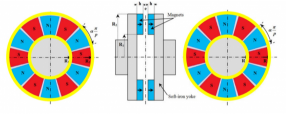
\includegraphics[scale=0.5]{PbGeometry2.png}
\end{figure}

Once again, if we compute $\mathbf{B}$ thanks to $\mathbf{A}$, and we replace it in $F_z$ expression, we get : 

\begin{equation*}
F_z = \dfrac{\pi\left(R_2^2-R_1^2\right)}{4\mu_0}\sum_{k=1}^{\infty}\left(\left(Z_k+X_k\right)^2-\left(W_k+Y_k\right)^2\right)    
\end{equation*}

Again, if we make the assumption where we keep only the first order harmonic, we have the following approached analytical expression for $F_z$ : 

\begin{equation*}
    F_z = \dfrac{8}{\pi}\dfrac{B^2_r}{\mu_0}R_2^2\left(1-\left(\dfrac{R_1}{R_2}\right)^2\right) \text{sin}^2\left(\alpha\dfrac{\pi}{2}\right)\dfrac{sh^2(a)}{sh(2(1+\nu)a)} \left(\text{cos}(p\delta)ch(2(1+\nu)a)+1\right)
\end{equation*}


\section{Results obtained with 2-D analytical model}
In this section will compute the magnetic field distribution in the air gap for different angular positions between the two discs for 6 pair of poles. We will analyze for each position the torque and axial force and then we will look at the influence of the number of pair of poles and the air-gap length on the coupling performances. 
\subsection*{No load condition}
\begin{figure}[H]
    \centering
    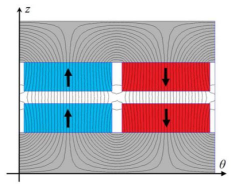
\includegraphics[scale=0.8]{config_d0.png}
\end{figure}
Let us analyze the results obtained with the 2-D analytical model. We first consider the case where the machine it at no-load: displacement angle delta =0.
We see that the magnetic flux lines are almost axial along the air gap and null between two neighbouring magnets.\\
Intuitively because the flux lines are aligned there will be no torque created because it is an equilibrium position for the magnets. If you put two magnets in front of each other they will not move transversely.\\
Mathematically we see that we have only a $B_{z}$ component for the flux and no $B_{\theta}$ component. We will thus have:
 For this position:
 \begin{enumerate}
     \item The torque is equal to zero
     \item Axial force is attractive and maximum
 \end{enumerate}
    \begin{align*}
 T_e = \dfrac{R_2^3-R_1^3}{3\mu_0}\int_0^{2\pi}B_z(\theta,z)B_{\theta}(\theta,z)d\theta
\end{align*}	
Torque depends on the products of $B_{\theta}$ and B$B_{z}$. The flux lines are here axial so we only have a $B_{z}$ component for the magnetic field and the product is equal to zero.
 \begin{align*}
    F_z =\dfrac{R_2^2-R_1^2}{4\mu_0}\int_0^{2\pi}\left(B^2_{IIz}(\theta,z)-B^2_{II\theta}(\theta,z)\right)d\theta
    \end{align*}
Axial force is maximal when $B_{z}$ is maximal and $B_{\theta}$ equal to zero. It is exactly the case here so we have the maximal attractive axial force possible. 
\subsection*{Full Load}
\begin{figure}[H]
    \centering
    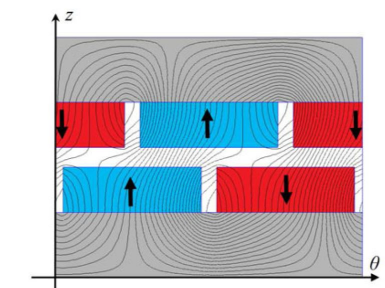
\includegraphics[scale=0.5]{config_d15.png}
\end{figure}
3)	We now consider the case where the machine is at full load: displacement angle delta = 15°.\\
We clearly observe the distortion of the flux lines due to the angular displacement of the magnets. For this angular position we have:
\begin{itemize}
    \item Maximum torque
    \item An attractive axial force
\end{itemize}
We have a maximal torque because we are at delta = pi/2p = 90/6 = 15° w$B_{\theta}$ different from zero at the same time so torque is greater than 0.\\
We have not the maximal axial force we have $B_{\theta}$ greater than 0 so $B_{z}^2$ – $B_{\theta}^2$is smaller than previously.

\subsection*{Magnets in opposition}
\begin{figure}[H]
    \centering
    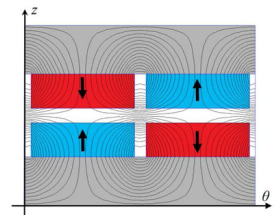
\includegraphics[scale=0.8]{config_d30.png}
\end{figure}
4)	We now consider the case where the magnets of the two discs are in opposed direction and the flux lines repel each other.\\
For this anglular position we have:
\begin{itemize}
    \item Torque equal to zero
    \item Repulsive axial force
\end{itemize}
We have a torque equal to zero because $B_{\theta}$ is always equal to zero so the product is equal to zero.\\
We have a repulsive axial force because $B_{\theta}^2$ is equal to zero and $B_{\theta}^2$ is greater than zero. The axial force is thus negative which means repulsive.

\subsection*{Torque in function of the displacement angle}
\begin{figure}[H]
    \centering
    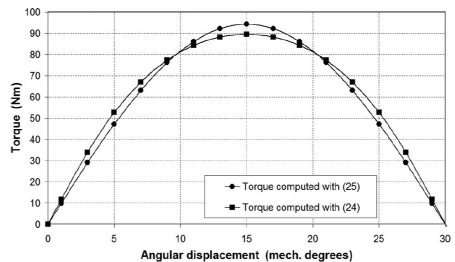
\includegraphics[scale=0.7]{Torque_d.png}
\end{figure}
This figure summarizes the variation of the torque in function of the angular displacement. We have the maximum torque at the half-pole pitch angle displacement and a torque equal to zero when the magnets are completely aligned or opposed.\\
The two curves represent the cases when we calculate with the first harmonic approximation and when we take the 10 first harmonics into account. There is less than 5$\%$ error between the two.

\subsection*{Axial force in function of the displacement angle}
\begin{figure}[H]
    \centering
    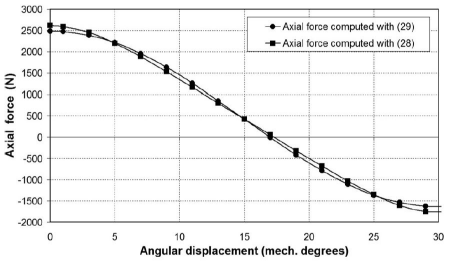
\includegraphics[scale=0.7]{axialf_d.png}
\end{figure}
This figure summarizes the variation of the axial force in function of the angular displacement. We have the maximum attractive axial force when the magnets are completely aligned and the maximum repulsive axial force when the magnets are completely opposed.

\subsection*{Influence of the air gap length}

The length of the air-gap has a huge influence on the performances of the magnetic coupling. More precisely, we will analyze its influence on the axial force and pull-out torque of the machine.
\begin{figure}[H]
    \centering
    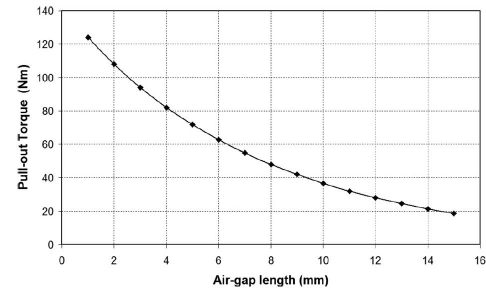
\includegraphics[scale=0.6]{airgap_t.png}
\end{figure}
We see that the pull-out torque due to the magnetic coupling decreases rapidly as the air-gap between the magnets increases. The maximum torque is almost divided by 2 when the air-gap increases from 2mm to 7mm.
\begin{figure}[H]
    \centering
    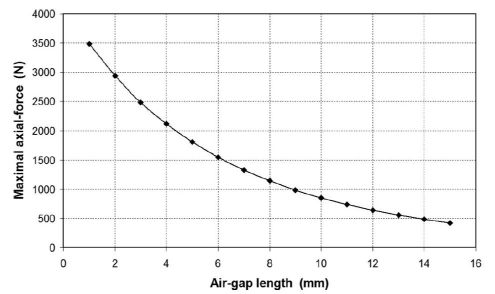
\includegraphics[scale=0.6]{airgap_f.png}
\end{figure}
We see that the axial force due to the magnetic coupling decreases rapidly as the air-gap length between the magnets increases.

\subsection*{Influence of the number of pole pairs}
The number of poles also has a big influence on the performances of the magnetic coupling. We will again analyze its effect on the pull-out torque and the axial force of the machine.
\begin{figure}[H]
    \centering
    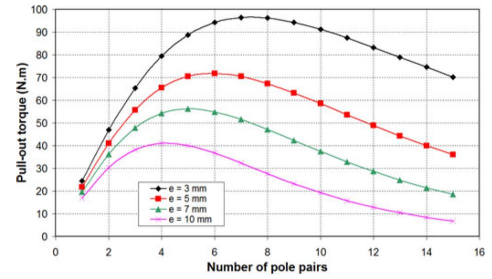
\includegraphics[scale=0.7]{poles_t.png}
\end{figure}
We see that the airgap length shift the optimal number of pole pairs to the right. But why does we have a non-monotonic influence of the poles pairs on the torque?\\
Magnetic torque is generated by the transversal coupling between south and north poles magnets. When we increase the number of poles we see that we have more transversal coupling between neighbouring magnets. So for now when we increase the number of poles the pull-out torque increases continuously (\textit{see FEM simulations in the slide! }).

But we also see that when the number of pole pairs increases, the magnetic field lines are more and more flattened. We have smaller values at the other side of the air-gap when the number of poles pairs increases. We have now that when the number of pole pairs increases the transversal coupling between north and south magnets at the opposite side of the air-gap decreases. 
This explains why we have first an increasing torque in function of the number of pole pairs and after a decreasing torque.
\begin{figure}[H]
    \centering
    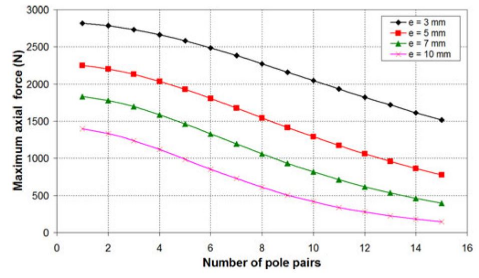
\includegraphics[scale=0.7]{poles_f.png}
\end{figure}
For the axial force we see that increasing the number of pole pairs always decreases the value of the axial force. This is because the axial force depends on the axial interaction between magnets at the opposite side of the air-gap. Increasing the number of poles pairs flattens the magnetic field and thus reduce the magnetic coupling between opposite magnets.

\subsection*{Synthesis of Section 5}
This analytical method is useful for:\\
1)Predict the effect of parameters on the coupling performances: 
\begin{itemize}
    \item 	increasing air-gap: decreases the pull out torque and the axial force
    \item increasing the number of pole pairs: non monotonic variation of pull out torque and decrease the axial force
\end{itemize}
2) Choose the optimum value of the number of pole pairs.


\section{Three-Dimensional FEM simulations and experimental results}

Both the FEM simulations and the experimental results (done with a real magnetic coupling) allow to show the limits of the analytical model created. Indeed, by analysing the influence of the air gap length as well as the number of pole pairs on the torque and axial force, it turns out that the model can give accurate results but not in all cases.

\bigskip

The main observations and conclusions are the following : 



%\begin{figure}[H]
%    \centering
%   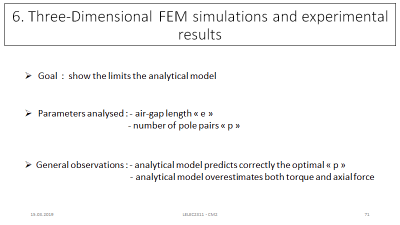
\includegraphics[scale=0.85]{Results_1.png}
%\end{figure}



\begin{itemize}
    \item The analytical model is very good at predicting the optimal number of pole pairs , when the air gap length is fixed. Optimal means here which gives the highest torque.
    \item In all cases, the analytical overestimates both torque and axial force.
    \item The difference between analytical model with first harmonic approximation (eq.25 in the paper) and the whole analytical expression (equ. 24 in the paper) for the torque and axial forces is very small.
    \item The error between analytical and FEM is lower for axial force than the one for torque
\end{itemize}





\appendix

\section{Solution of \texorpdfstring{$A^{\rm III}$}{A} using variable separation}
\label{apdxA}

The solution $A^{\rm III}$ is decomposed into :
$$A_{\rm III} = A_{\rm III, z}\, A_{\rm III, \theta}$$
Solving with $z$ :
$$\dfrac{1}{R_e^2}\, \dfrac{\partial^2 A_{\rm III}}{\partial \theta ^2}
+ \underbrace{ \dfrac{\partial^2 A_{\rm III}}{\partial z^2}}
= -\dfrac{\mu_0}{R_e}\, \dfrac{\partial M_z}{\partial \theta}
\hspace{.5cm} \text{for}
\left\{
\begin{array}{lll}
& h+e \leq z \leq 2h+e \\
& 0 \leq \theta \leq 2\pi/p
 \end{array}
\right. 
$$
$$ \dfrac{\partial^2 A_{\rm III}}{\partial z^2} = k^2 \quad \longrightarrow \quad A_{\rm III,\ z} = Z(z) \quad \longrightarrow \quad Z'' = k^2 $$
Yet, we are looking for a solution of the type $Z_k = \cosh (kz)$ which is solution of $\dfrac{Z''}{Z} = k^2$. We will therefore set a correcting coefficient to make our solution match with the real ODE :
$$Z_k = a_k\, \cosh(kz) + \underbrace{c_k}_{\text{correcting coeff}}$$
\noindent 
Solving with $\theta$ :
$$ \underbrace{\dfrac{1}{R_e^2}\, \dfrac{\partial^2 A_{\rm III}}{\partial \theta ^2}}
+ \dfrac{\partial^2 A_{\rm III}}{\partial z^2}
= \underbrace{-\dfrac{\mu_0}{R_e}\, \dfrac{\partial M_z}{\partial \theta}}
\hspace{.5cm} \text{for}
\left\{
\begin{array}{lll}
& h+e \leq z \leq 2h+e \\
& 0 \leq \theta \leq 2\pi/p
 \end{array}
\right. $$
$$ \dfrac{1}{R_e^2}\, \dfrac{\partial^2 A_{\rm III}}{\partial \theta ^2}
= -\dfrac{\mu_0}{R_e}\, \dfrac{\partial M_z}{\partial \theta} \quad \longrightarrow \quad A_{\rm III,\ \theta} = \Theta(\theta) \quad \longrightarrow \quad \dfrac{1}{R_e^2} \Theta'' = -\dfrac{\mu_0}{R_e} \dfrac{\partial M_z}{\partial \theta} $$
\begin{align*}
     \dfrac{1}{R_e^2} \Theta'' &= -\dfrac{\mu_0}{R_e} \sum\limits_{k=1}^{\infty}
M_k\ \left( \cos(kp\theta)\, \cos(kp\delta) + \sin(kp\theta)\, \sin(kp\delta) \right)\, kp  \numberthis{} \label{eq:TH}\\
 \Theta &= \sum\limits_{k=1}^{\infty} K_k \left( \cos(kp\theta)\, \cos(kp\delta) + \sin(kp\theta)\, \sin(kp\delta) \right)
\end{align*}
To find $K_k$ we reintroduce $\Theta$ in equation (\ref{eq:TH}).
\begin{align*}
& - \dfrac{1}{R_e^2} K_k \sum\limits_{k=1}^{\infty} \left( \cos(kp\theta)\, \cos(kp\delta) + \sin(kp\theta)\, \sin(kp\delta) \right)\, (kp)^2 \\
&= -\dfrac{\mu_0}{R_e}\, \sum\limits_{k=1}^{\infty} M_k\, \left( \cos(kp\theta)\, \cos(kp\delta) + \sin(kp\theta)\, \sin(kp\delta) \right) kp 
\end{align*}
And find : 
$$ K_k = \mu_0\dfrac{R_e}{kp}M_k$$

We have then:
\begin{align*}
A_{\rm III} &= A_{\rm III, z}\, A_{\rm III, \theta} \\
&= \sum\limits_{k=1}^{\infty} \left( a_k\, \cosh(kz) + c_k \right)\,K_k \left( \cos(kp\theta)\, \cos(kp\delta) +
\sin(kp\theta)\, \sin(kp\delta) \right) \\
&= \sum\limits_{k=1}^{\infty} \left( b_k\, \cosh(kz) + 1 \right)\,K_k \left( \cos(kp\theta)\, \cos(kp\delta) +
\sin(kp\theta)\, \sin(kp\delta) \right) \\
&= \sum\limits_{k=1}^{\infty} \left( b_k\, \cosh(kz) + 1 \right)\,K_k \cos(kp\theta)\, \cos(kp\delta) + \sum\limits_{k=1}^{\infty} \left( b_k\, \cosh(kz) + 1 \right)\,K_k \sin(kp\theta)\, \sin(kp\delta)  \\
&= \sum\limits_{k=1}^{\infty}\Bigr( \cosh(kz)\, \underbrace{ b_k\, K_k\, \cos(kp\delta)}_{d_k} + K_k\, \cos(kp\delta) \Bigr)\, \cos(kp\theta) \\
&+ \sum\limits_{k=1}^{\infty}\Bigr( \cosh(kz)\, \underbrace{ b_k\, K_k\, \sin(kp\delta)}_{e_k} + K_k\, \sin(kp\delta) \Bigr)\, \sin(kp\theta) \numberthis{} \label{eq:tsb}
\end{align*}
\noindent
In order to determine the coefficients $d_k$ and $c_k$, we should use the condition (\ref{eq:BC2_2}) i.e $\dfrac{\partial A_{\rm III}}{\partial z}\Bigr\rvert_{z = 2h+e} = 0$. This relation suggests that our solution should behave in $$\cosh(\alpha(z-2h-e))$$ such that $$\left( \cosh(\alpha(z-2h-e)) \right)'\Bigr\rvert_{z = 2h+e} = 0.$$ We thus simply introduce this in (\ref{eq:tsb})
\begin{align*}
 A_{\rm III} =& \sum\limits_{k=1}^{\infty}\Bigr( \cosh(\alpha\, (z-2h-e)) \Bigr)\,
d_k + K_k\, \cos(kp\delta) \Bigr)\, \cos(kp\theta) 
\\&+ \sum\limits_{k=1}^{\infty}\Bigr( \cosh(\alpha\, (z-2h-e))\,
e_k + K_k\, \sin(kp\delta) \Bigr)\, \sin(kp\theta)
\end{align*}
$\alpha$ is found by reintroducing this solution into the original Poisson equation (\ref{eq:PoissonIII}) : $\alpha = \dfrac{kp}{R_e}$
\begin{align*}
A_{\rm III} (\theta, z) 
&= \sum\limits_{k=1}^{\infty}\Bigr( \cosh \bigr((kp/R_e)\, (z-2h-e)\bigr) \Bigr)\,
d_k + K_k\, \cos(kp\delta) \Bigr)\, \cos(kp\theta) \\
&+ \sum\limits_{k=1}^{\infty}\Bigr( \cosh \bigr((kp/R_e)\, (z-2h-e)\bigr) \Bigr)\,
e_k + K_k\, \sin(kp\delta) \Bigr)\, \sin(kp\theta)
\end{align*}

The article solution is the same except for different constants definitions. We will still use the former as we should align on this solution.

\begin{align*}
A_{\rm III} (\theta, z) 
&= \sum\limits_{k=1}^{\infty} a_k^{\rm II}\ \dfrac{ch((kp/R_e)(z-2h-e))}{ch((kp/R_e)h)}
+ K_k\, \cos(kp\delta) \Bigr)\, \cos(kp\theta) \\
&+ \sum\limits_{k=1}^{\infty} c_k^{\rm II}\ \dfrac{ch((kp/R_e)(z-2h-e))}{ch((kp/R_e)h)}
+ K_k\, \sin(kp\delta) \Bigr)\, \sin(kp\theta)
\end{align*}

The integration constants $a_k^{\rm III}$ and $c_k^{\rm III}$ are determined using a Fourier series expansion and the condition (\ref{eq:BC2_1}).

\begin{align*}
A_{\rm III}(\theta, h+e) &= 
\sum\limits_{k=1}^{\infty} \Biggr( 
a_k^{\rm III}\, \dfrac{ch((kp/R_e)h))}{ch((kp/R_e)h)}
+ K_k\, \cos(kp\delta) \Biggr)\, \cos(kp\theta) \\
&+ \sum\limits_{k=1}^{\infty} \Biggr( 
c_k^{\rm III}\, \dfrac{ch((kp/R_e)h))}{ch((kp/R_e)h)} 
+ K_k\, \sin(kp\delta) \Biggr)\, \sin(kp\theta) \\
A_{\rm III}(\theta, h+e) &= \sum\limits_{k=1}^{\infty} \underbrace{\left( a_k^{\rm III}\,+ K_k\, \cos(kp\delta) \right)}_{a_k}\, \cos(kp\theta) \\
&+ \sum\limits_{k=1}^{\infty}\underbrace{ \left( c_k^{\rm III}\,+ K_k\, \sin(kp\delta) \right)}_{b_k}\, \sin(kp\theta) = A_{\rm II}(\theta, h+e) 
\end{align*}

\underline{Reminder Fourier series expansion :}

A Fourier series is a representation of a periodic function as a sum of orthogonal sinusoids, each with an integer number of cycles in the period of the function. In general, the series has an infinite number of such harmonics. 
\footnote{\url{https://en.wikipedia.org/wiki/Fourier_series}}
\begin{align*}
a_0 := \dfrac{2}{L} \int_{0}^{L} f(t)\, dt \hspace{1cm}
a_n &:= \dfrac{2}{L} \int_{0}^{L} f(t)\, \cos(nt) dt \hspace{1cm}
b_n := \dfrac{2}{L} \int_{0}^{L} f(t)\, \sin(nt) dt \\
f(t) &\sim \dfrac{1}{2}a_0+\sum\limits_{n=1}^{\infty} \left[ a_n\, \cos(nt) + b_n\, \sin(nt) \right]
\end{align*}

In our case :
\begin{align*}
f(t) &= A_{\rm II}(\theta,h+e) \hspace{1cm} &
L &= \dfrac{2\pi}{p} &
a_k &= a_n &
b_k &= b_n 
\end{align*}

We then find :
\begin{align*}
a_k + K_k\, \cos(kp\delta) &= \dfrac{2p}{2\pi}\, \int_0^{2\pi/p} A_{\rm II} (\theta,h+e)\, \cos(kp\theta)\, d\theta \\
b_k + K_k\, \sin(kp\delta) &= \dfrac{2p}{2\pi}\, \int_0^{2\pi/p} \underbrace{A_{\rm II} (\theta,h+e)}_{?}\, \sin(kp\theta)\, d\theta 
\end{align*}

We notice that solving these coefficients leads to find the expression of $A$ in region \rm II. This means solving the Laplace equation in the air gap. This in turns means finding $A$ in region \rm I.

\section{Coefficient for \texorpdfstring{$\mathbf{A}$}{A}}

\begin{equation*}
\begin{split} 
X_k = & ~~~ c_k^{II} \dfrac{ch((kp/R_e)(\zeta - h -e))}{sh((kp/R_e)e)} \\ & - d_k^{II}\dfrac{R_e}{kp}\dfrac{ch((kp/R_e)(\zeta -e))}{sh((kp/R_e)e)} \\
\end{split}
\end{equation*}

\begin{equation*}
\begin{split} 
Y_k = & - c_k^{II} \dfrac{sh((kp/R_e)(\zeta - h -e))}{sh((kp/R_e)e)} \\ & + d_k^{II}\dfrac{R_e}{kp}\dfrac{sh((kp/R_e)(\zeta -e))}{sh((kp/R_e)e)} \\
\end{split}
\end{equation*}

\begin{equation*}
\begin{split} 
Z_k = & - a_k^{II} \dfrac{ch((kp/R_e)(\zeta - h -e))}{sh((kp/R_e)e)} \\ & + b_k^{II}\dfrac{ch((kp/R_e)(\zeta -e))}{sh((kp/R_e)e)} \\
\end{split}
\end{equation*}

\label{apdxB}

\section{Vector potential}

The following demonstration was provided by assistant Guillaume François: 

\begin{figure}[H]
    \centering
    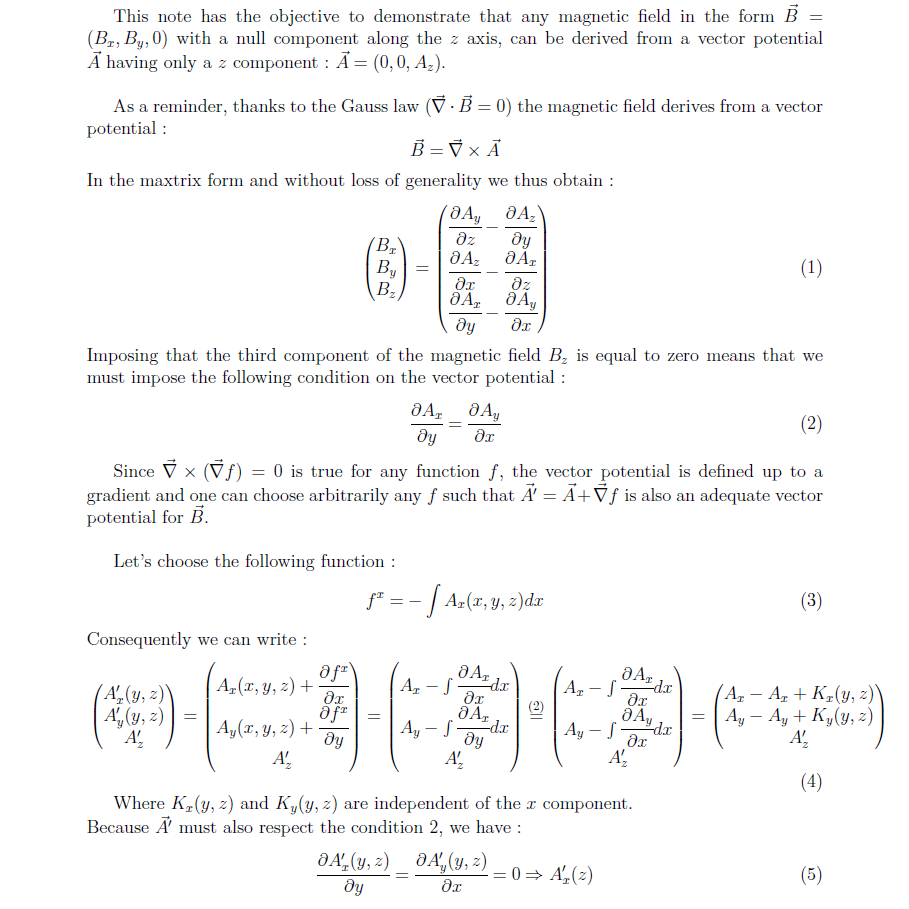
\includegraphics[scale=0.6]{VectPot1.png}
\end{figure}
\begin{figure}[H]
    \centering
    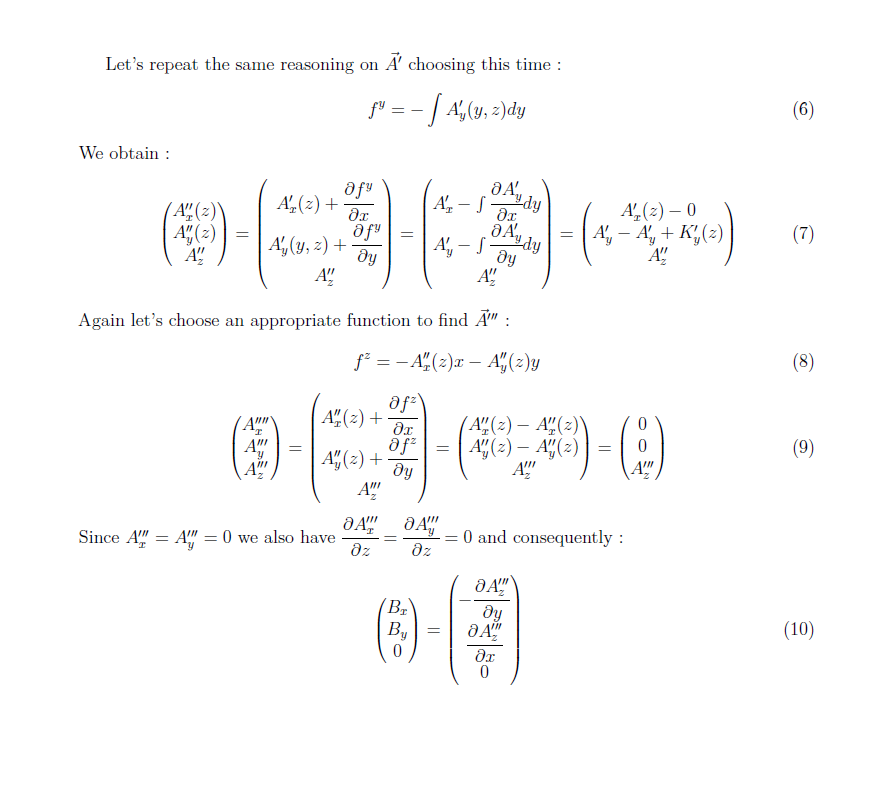
\includegraphics[scale = 0.6]{VectPot2.png}
\end{figure}
\label{apdxC}

\unappendix
